\section{Background estimation: jet faking photons}
\label{sec:bkg:estimation}

It was discussed in \Ch{\ref{ch:strategy}} that the main backgrounds encountered for this analysis are those in which there is at least a photon and a jet in the final state. Although \ac{SM} \gammajet events (prompt photons discussed in \Sect{\ref{subsec:theory:sm:prompt_photon}}) is the dominant background, jet faking photons events is another important source of background that need to be taken into account.

% Emphasizing again, backgrounds in this analysis are only estimated to optimise the modeling of it, that is, finding the most optimal function that can describe it, henceforth, not involving them in the final calculations with data. \fixme{add this?}


Jets can be misidentified as photons (fake photons) if they fluctuate to \pizero's (in a dominant way), resulting in an \ac{EM} object indistinguishable from a single, real, highly energetic photon (also called prompt photon). To cope with the large jet backgrounds, the \texttt{Tight} identification criteria is applied on photon candidates. This selection is expected to contain prompt photons with moderate jet contamination. As this misidentification rate is not expected to be accurately modeled in \ac{MC}, a data-driven determination has been used. The \texttt{Tight} offline identification is by design tighter than the photon trigger used to collect the data, so there are quite a few photon candidates from jets that will fail the \texttt{Tight} \ac{WP} but satisfy some intermediate selection. These photon-like jets, from hereinafter called pseudo-photons (or \texttt{Non-Tight}), are defined as those passing the \texttt{Loose} identification but failing (at least) one of \wone, \fside, \deltae, \eratio \texttt{Tight} selection cuts \cite{ATLAS-EGamma-Performance-2015-2017}.

To estimate the number of jet faking photons in the signal regions of the present analysis a combination of two methods is employed. Using the so-called ABCD method with the different expected isolation profiles for both real and fake photons, it is possible to estimate fake factors that allow the calculation of the fakes in signal regions~\cite{ATLAS-SUSY-PhotonMetX-13TeV,ATLAS-SUSY-PhotonMetX-13TeV-NOTE,ATLAS-SUSY-PhotonJetMet-13TeV,ATLAS-SUSY-PhotonJetMet-13TeV-NOTE}. The second method, by making use of a sequential template-fit procedure to the photon isolation distribution in data and \ac{MC}, allows to correctly count the number of real and fake photons in the regions delimited by the ABCD method.

\begin{table}[ht!]
    \centering
    \caption{Baseline event selection used for the jet fakes estimation using the template fit procedure. \ptiso is defined as shown in \Eqn{\ref{eq:objects:egamma:iso:definitions}}.\fixme{revise selection on jet pt}}
    \begin{tabular}{| l | c |}
        \hline
                                        & Selection \\ \hline
        Trigger                         & HLT\_g140\_loose \\ \hline
        \ngamma                         & \(\ge1\) \\ \hline
        \ptgam [GeV]                    & \(>150\) \\ \hline
        \ptjet [GeV]                    & \(> 60\) \\ \hline
        \njets                          & \(>0\) \\ \hline
        \nlep                           & \(0\) \\ \hline
        Track isolation                 & \(\ptiso < 0.05\) \\ \hline
        \(|\etagam|\) acceptance region & \etagamacc \\ \hline
        \myj [GeV]                      & \(\myj > 500\) \\ \hline
    \end{tabular}
    \label{tab:bkg:estimation:selection}
\end{table}

The study uses \texttt{Loose} identification and non-isolated photons and the event selection taking part in this study is shown in \Tab{\ref{tab:bkg:estimation:selection}}.
It is important to notice that the \texttt{Tight} and isolated photons used in the search are only a sub-set of those used in this background-estimation study. By requiring the \texttt{Loose}, non-isolated, photons to pass the selection shown in \Tab{\ref{tab:bkg:estimation:selection}}, \texttt{Tight} identification and \(\etiso < 0 ~\gev\) (see \Eqn{\ref{eq:objects:egamma:iso:definitions}}), one recovers the \texttt{Tight} and isolated photons used in the search.
Finally, a manual Overlap-Removal procedure is carried out between the photons and jets, to remove jet overlapping with the leading \texttt{Loose} photon if \(\dryj<0.4\).
This method, as previously mentioned, is data-driven. Given that unblinding of the full Run-2 data is not performed up to the last analysis stage, only the 2015+2016 dataset is used, as it was already unblinded in a previous work by the \ac{ATLAS} collaboration~\cite{ATLAS-PhotonJetResonances-2016}.


\subsection{ABCD method}
\label{subsec:bkg:estimation:abcd}

The ABCD method defines a signal region \(A\) and three control regions, namely \(B\), \(C\) and \(D\).
These regions are defined by varying the identification status between \texttt{Tight} and \texttt{Non-Tight}, and also by changing the calorimetric isolation requirements (isolated and non-isolated)~\cite{ATLAS-EXOTICS-Monophoton-2017}.
The complete definition of the ABCD regions is given as:
\begin{itemize}
    \item Region \(A\): \texttt{Tight} photons and \(-20 < \etiso < 0~ \gev\)
    \item Region \(B\): \texttt{Tight} photons and \(8 < \etiso < 80~ \gev\)
    \item Region \(C\): \texttt{Non-Tight} photons and \(-20 < \etiso < 0~ \gev\)
    \item Region \(D\): \texttt{Non-Tight} photon and \(8 < \etiso < 80~ \gev\)
\end{itemize}
where \etiso was defined in \Eqn{\ref{eq:objects:egamma:iso:definitions}}. \Fig{\ref{fig:bkg:estimation:abcd:diagram}} shows the resulting four different regions.

\begin{figure*}[ht!]
    \centering
    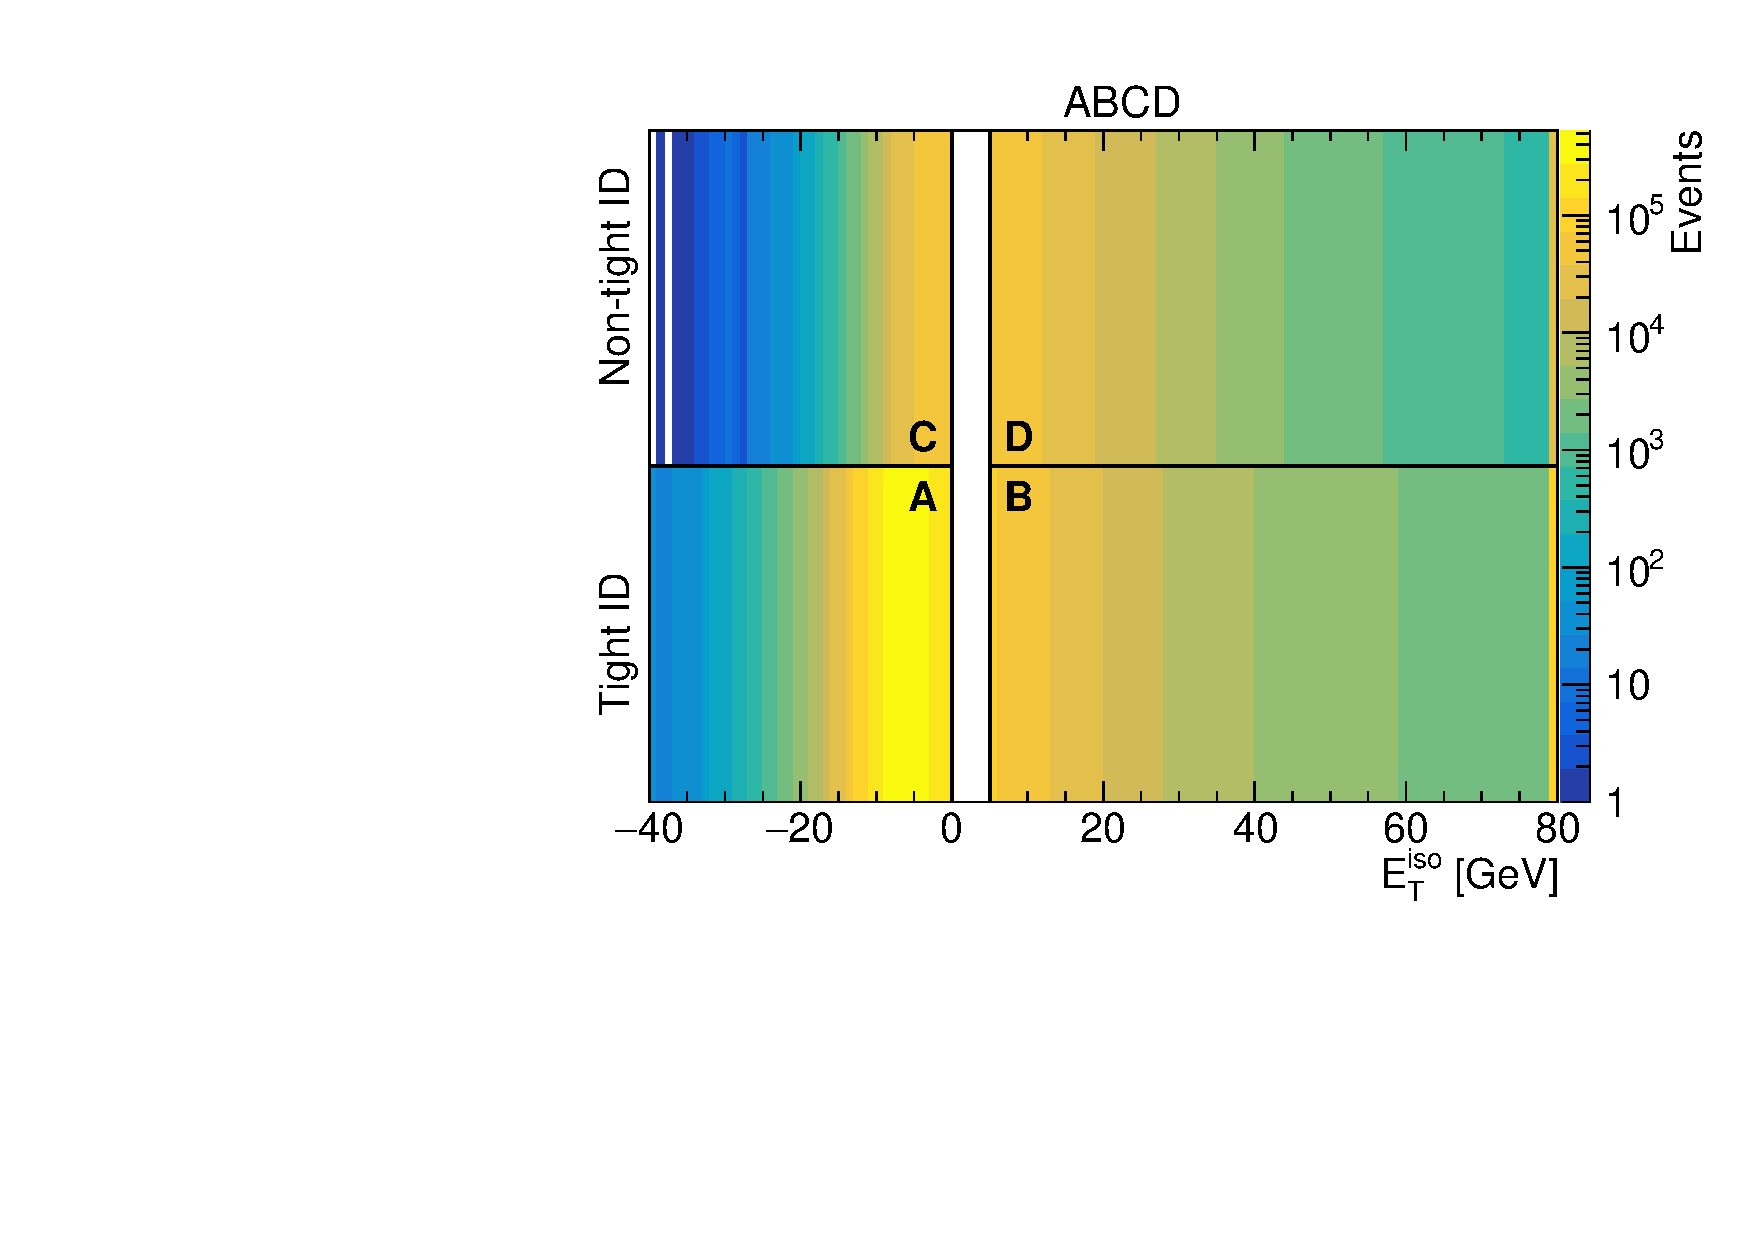
\includegraphics[width=0.65\textwidth]{5_resonances/bkg/estimation/ABCD_data_regions}
    \caption{Identification vs. \(\etiso\) two-dimensional distribution from data events for the Full Run-2 dataset.}
    \label{fig:bkg:estimation:abcd:diagram}
\end{figure*}

Assuming that there is no signal contamination in any control region, the \(B\), \(C\) and \(D\) regions are only composed of background \(N_{(B,C,D)}=N^{b}_{(B,C,D)}\). In addition assuming no correlation between isolation and the considered shape variables, the following relation holds: \(N^{b}_{B}/N^{b}_{A}=N^{b}_{D}/N^{b}_{C}\). Moreover, two different \acp{FaF} could be defined:
\begin{equation*}
    \ffiso = \frac{N_{C}}{N_{D}} \qquad \ffid = \frac{N_{B}}{N_{D}}
\end{equation*}
Therefore, the number of jets faking photons can be estimated using the \ac{FaF} as:
\begin{equation}
    \label{eq:bkg:estimation:abcd:njfakes}
    N_{\jfake} = N_{A} = \ffiso \times N_{B}  = \ffid \times N_{C}.
\end{equation}

So two different approaches could be used: to model the fake photons using the \texttt{Tight} but non isolated photons from region \(B\) using \ffiso or model the fake photons using the \texttt{Non-Tight} but isolated photons using the \ffid.
Even though both approaches give equivalent results, the \ffiso approach is used as it leads to higher statistics.
%the systematic uncertainties are found to be lower.

Using the \ac{FaF}, now it is possible to estimate the jet-faking photons background contribution in each region of the analysis (\(R\)). To this end, a jet control region (CRJ-R) is defined equally to the region \(R\) but replacing the isolation requirements with the one used in region \(B\), and weighted by the corresponding \ffiso:
\begin{equation*}
    N^{R}_{\jfake}(\pt) = \ffiso(\pt)\cdot N_{\text{CRJ-R}}(\pt)
\end{equation*}





\subsection{Corrections to the ABCD method}
\label{subsec:bkg:estimation:abcd_corrections}

Several corrections can be applied to the ABCD method.
The first one is to consider the possibility of a signal contamination in any of the control regions \(B\), \(C\) or \(D\). By subtracting the amount of signal events in these regions, \Eqn{\ref{eq:bkg:estimation:abcd:njfakes}} becomes:
\begin{equation}
    \label{eq:bkg:estimation:abcd_corrections:njfakes_leak}
    N_{\jfake} = \frac{N_{B} - N_{B}^{s}}{N_{D} - N_{D}^{s}} \times (N_{C} - N_{C}^{s})
\end{equation}
where \(N_{(B,C,D)}^{s}\) is the number of real photons in each region. The estimation of these numbers is a complicated task, since it is needed to have a correct description of the real photons in data, and it is highly contaminated with fake photons. The calculation of the number of real photons in data is performed with an iterative template fit method to the calorimetric isolation distribution in data, explained in more detail below.


The presence of a residual correlation of the background across the four regions, which may manifest itself as a difference in the background distributions for the \texttt{Tight} and \texttt{Non-Tight} regions could be taken into account by calculating:
\begin{equation*}
    R = \frac{N^{b}_{A}\,N^{b}_{D}}{N^{b}_{B}\,N^{b}_{C}} \neq 1.
\end{equation*}

However, since \(R\) can not be found in data because that would mean to obtain \(N_A\), an equivalent parameter is calculated, which can also be written using real photons (leakage photons) subtraction:

\begin{equation*}
    R' = \frac{N_{A'}\,N_{D'}}{N_{B'}\,N_{C'}} = \frac{(N_{A'} - N^{s}_{A'})\,(N_{D'}-N^s_{D'})}{(N_{B'}-N^s_{B'})\,(N_{C'}-N^s_{C'})}
\end{equation*}
with the definition for each primed region being:
\begin{itemize}
    \item region \(A'\): \texttt{Tight} photons and \(8 < \etiso < 15~ \gev\).
    \item region \(B'\): \texttt{Tight} photons and \(16 < \etiso < 80~ \gev\).
    \item region \(C'\): \texttt{Non-Tight} photons and \(8 < \etiso < 15~ \gev\).
    \item region \(D'\): \texttt{Non-Tight} photons and \(16 < \etiso < 80~ \gev\).
\end{itemize}


The particular selection of 8 \gev\ aims to define a background only region, but keeping enough statistics to compute the \(R'\) values. In \Fig{\ref{fig:bkg:estimation:abcd_corrections:rprime}} the \(R'\) values are shown as a function of \ptgam.
The values are very close to 1 with some exceptions in which the values deviate from 1 by a maximum amount of \(\approx 20\%\) at low \ptgam.
\begin{figure}[htbp]
    \centering
    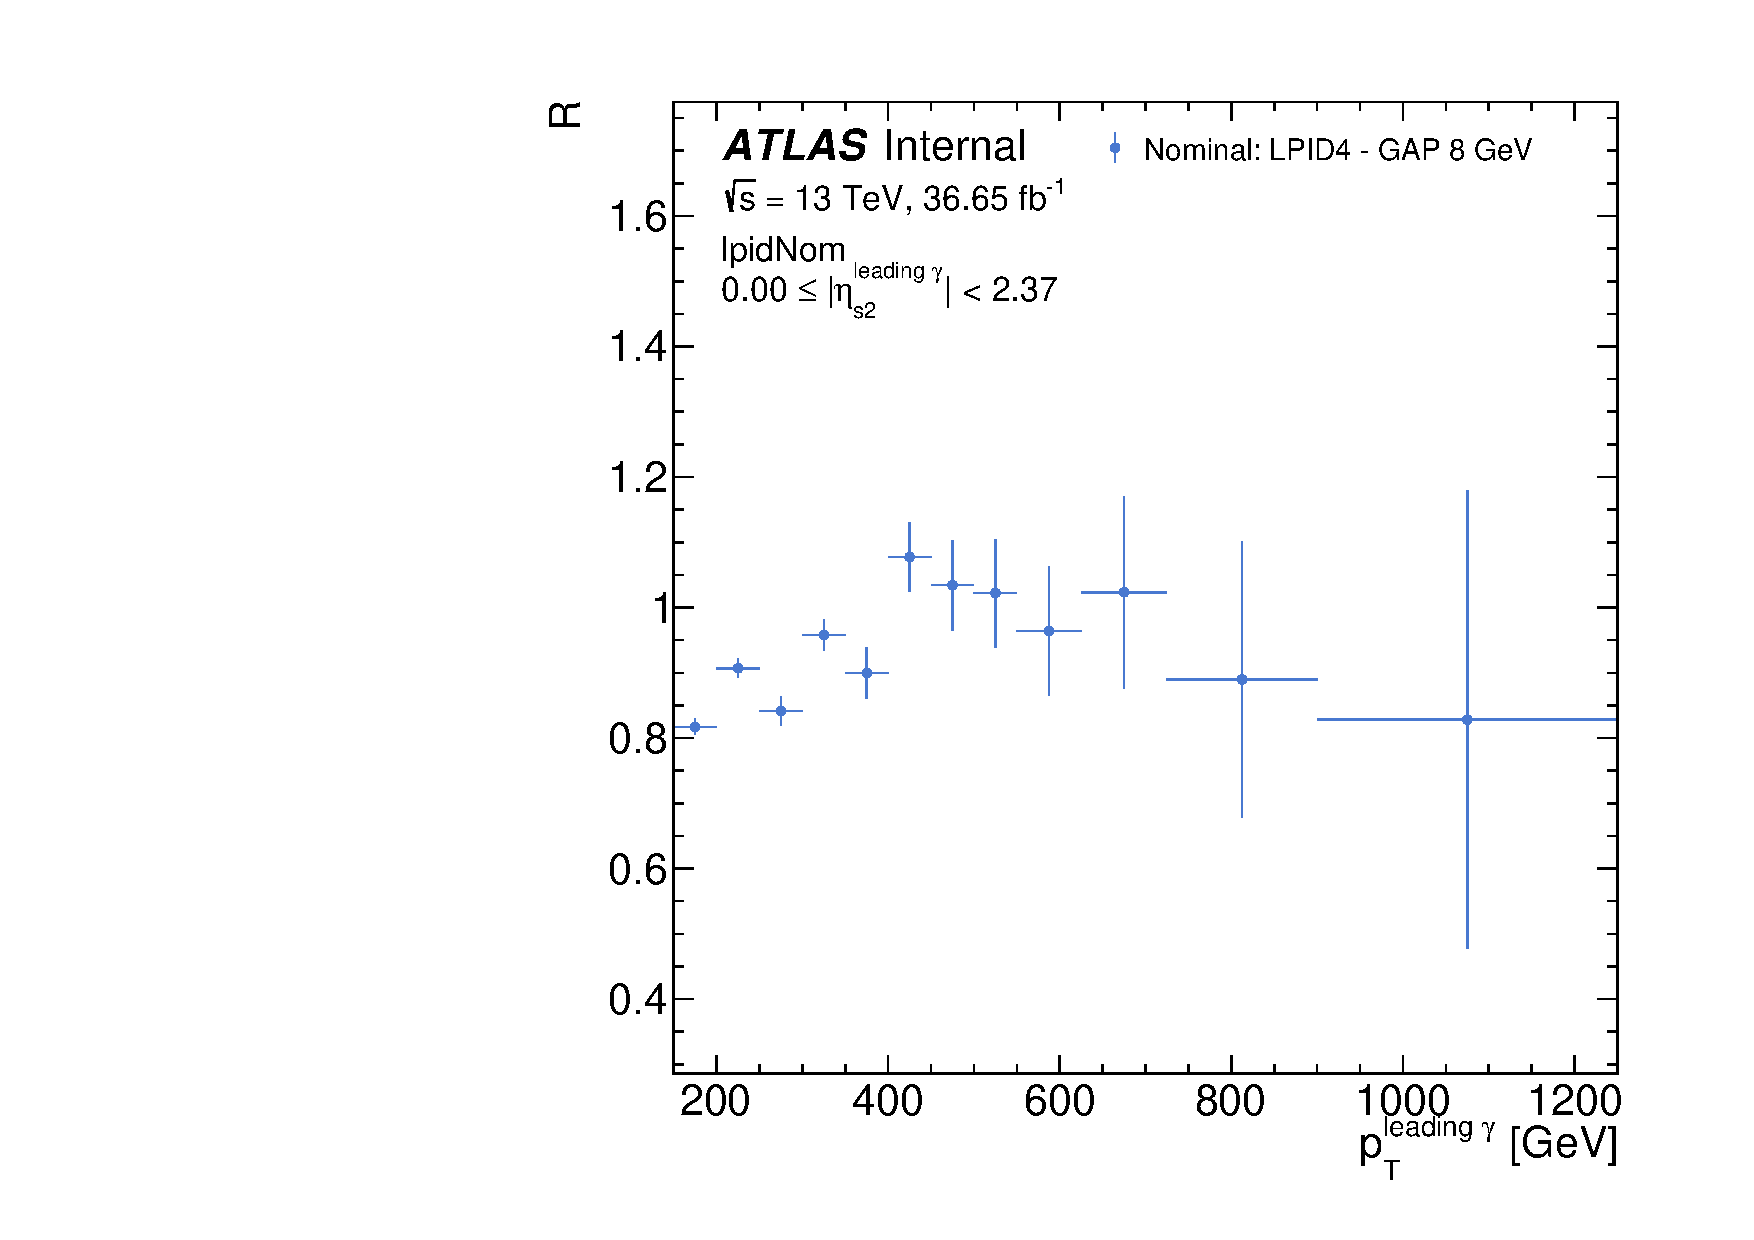
\includegraphics[width=0.5\linewidth]{5_resonances/bkg/estimation/coefficients/can__R__lpidNom__lph_pt0__abslph_etas20_0__2015_2016}
    \caption{\(R'\) values computed as a function of \ptgam. The error bars shown correspond to the statistical uncertainties.}
    \label{fig:bkg:estimation:abcd_corrections:rprime}
\end{figure}



Finally, taking into account the leakage and possible correlations, the \Eqn{\ref{eq:bkg:estimation:abcd_corrections:njfakes_leak}} for the expected number of jet fakes results:
\begin{equation}
    \label{eq:bkg:estimation:abcd_corrections_ffiso}
    N_{\jfake}(\pt) =
    N^{b}_{A} =
    \left[R'  \frac{N_{C}-N^{s}_{C}}{N_{D}-N^{s}_{D}}  \left(1 - \frac{N^{s}_{B}}{N_{B}} \right)\right] \times N_B = \ffiso(\pt)  \times  N_{B}(\pt).
\end{equation}

% In case of working with \ffiso, the systematic uncertainties are evaluated by varying the definition of the \texttt{Non-Tight} objects, namely the \textit{tight-3} (failing at least one of \(w_{s3}\), \fside, \deltae) and \textit{tight-5} (failing at least one of \(w_{s3}\), \fside, \deltae, \eratio and \wstot). On the other hand, for \ffid, systematic variations correspond to change the gap set between regions \(A\) and \(C\) with \(B\) and \(D\). In the nominal case the gap is of \(8~\gev\) and the variations correspond to gaps of 5 and \(11~\gev\). As another systematic variation, for both types of fake factors, to account for the differences introduced by the residual correlation between regions, \(R'\) is set to 1, and it is also calculated using the number of fake photons (instead of data with signal leakage).




\subsection{Template fits procedure}
\label{subsec:bkg:estimation:fits}


In order to estimate the number of jet faking photons in the signal regions of the analysis, it is necessary to have an estimate on the number of events with real photons in the ABCD control regions \(B\), \(C\) and \(D\). To achieve this, a series of fits to the data and real-photon \ac{MC} photon isolation distribution is carried out for both \texttt{Tight} and \texttt{Non-Tight} photons. The final objective of the iterative fits, is to have real- and fake-photon components fits to the data distribution, that will then be used to compute the number of real photons in the ABCD control regions. The procedure uses the \ac{MC} \pythia samples, which are expected to be real photons, hence the leak photon contribution will be very small. The calculation is performed in 11 \ptgam bins:
\[
    \ptgam: \left[ 150, 200, 250, 300, 350, 400, 450, 500, 550, 625, 725, 900, \infty \right]~\gev.
\]


The shape of the calorimetric isolation \etiso is fitted in an iterative fashion, using photons passing the \texttt{Tight} and loose-prime \texttt{Non-Tight} identification criteria, as explained above. 
By definition, events with \(\etiso<0~\gev\) pass the calorimetric isolation requirement and correspond to photons falling in region \(A\) if they are \texttt{Tight}, or \(C\) if they are \texttt{Non-Tight}. On the other hand, events with \(\etiso>0~\gev\) define regions \(B\) (\texttt{Tight} photons) and \(D\) (\texttt{Non-Tight} photons).
In what follows, real photons leaked into the \texttt{Non-Tight} regions will referred as leaked photons. Both \texttt{Tight} and \texttt{Non-Tight} photons will contain a fake component, which will dominate over the leaked photons in the latter case~\cite{ATLAS-DiPhotonSearchIsolation-NOTE,ATLAS-EleMuPhoIsolation-NOTE}.

The sequence of fits proceeds as follows:
\begin{enumerate}
    \item \underline{\texttt{Tight} \ac{MC} photons fit}: Given prompt photon samples provides a good description of \texttt{Tight} photons, its \etiso distribution is fitted with a \ac{CBall} function\footnote{This function consists of a Gaussian core but one of the tails of it follows a power-law form. This function was named after the Crystal Ball Collaboration.}. It was found that the simple \ac{CBall} desription does not accomodate well in the whole range, specially in the bulk of the \etiso distribution, therefore a more flexible function is employed. In this way, an improved version of the \ac{CBall} is used, namely the \ac{DSACB} function\footnote{As it names suggests, in the \ac{DSACB} function, the two tails are modeled by power-law functions, and the core of the Gaussian distribution has two different standard deviations, hence the asymmetry.}. Although the description is much better in this case, the Gaussian core struggles to model correctly the peak of the distribution.
    \item \underline{\texttt{Non-Tight} data leak subtraction}: Using the leak photon component from \ac{MC}, the fake photon shape is estimated by subtracting the leak photons histogram to data in the whole \etiso range. This provides a very good description of the fake photon component in the \texttt{Non-Tight} region.
    \item \underline{\texttt{Tight} data composite fit}: Using the real photons \ac{DSACB} shape estimated in the first step and the fake photons shape estimated in the previous step, a composite fit is performed to the \texttt{Tight} photons \etiso distribtution in data. An example of the resulting fit in three different \pt-bins is shown in \Fig{\ref{fig:bkg:estimation:fits_tightID_data}}.

        The final composite distribution is in good agreement with data, indicating the correct selection of the distributions for each component. The real photons component is the responsible for the high peak at low isolation values, while the fake components contributes mainly in the range \(0~\gev < \etiso < 40 ~\gev\), but having a much smaller yield, as expected. Some differences between the model and data can be seen near the peak of the distribution, as indicate by the fit pull. This difference was also seen in the first step of the calculation when modeling the real photon components, and it is directly originating from the gaussian modeling of the real photons peak.

        \begin{figure}[bth!]
            \centering
            \begin{subfigure}[h]{0.32\linewidth}
                \centering
                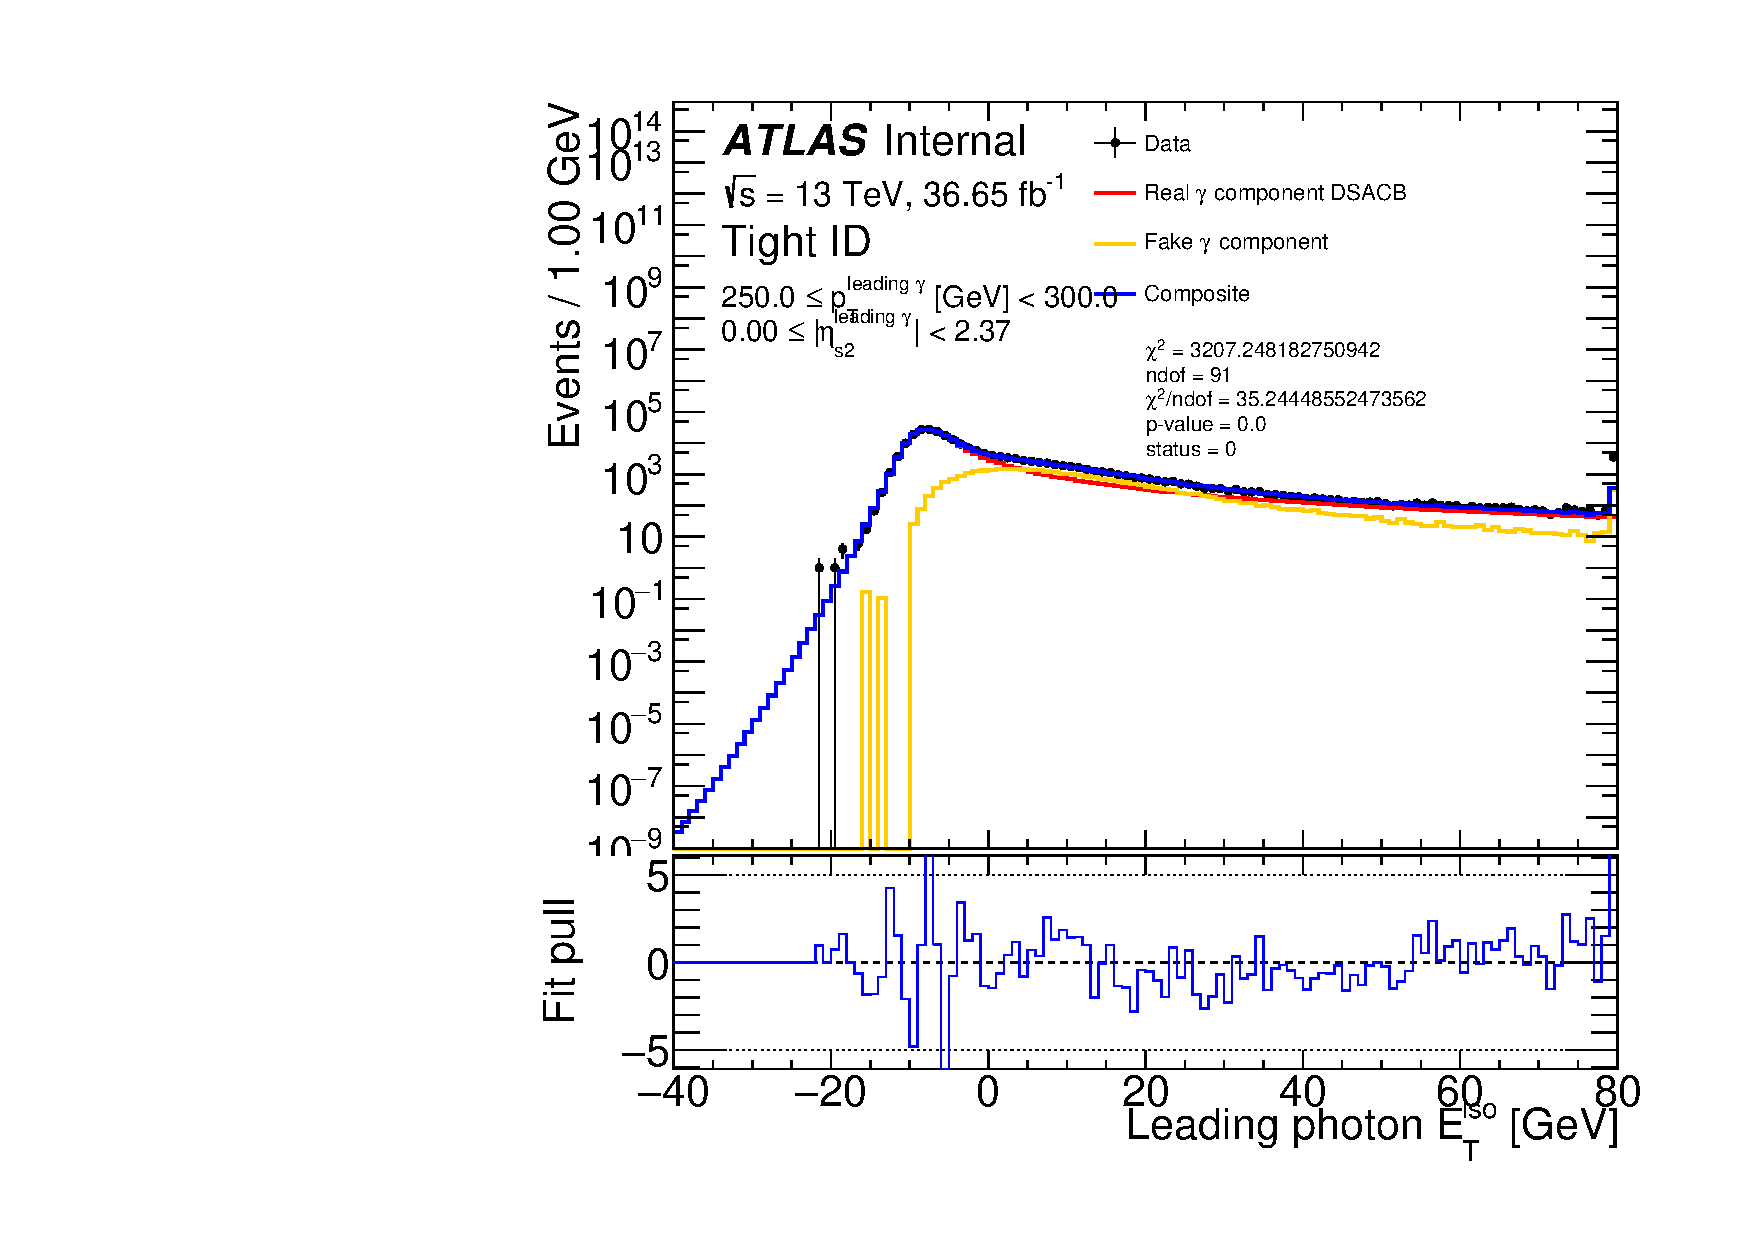
\includegraphics[width=\linewidth]{5_resonances/bkg/estimation/fits/lpid4/2015_2016/lph_pt0/lph_pt0__250p0/data__tight__composite__lph_pt0__250p0__abslph_etas20__0p00}
                \caption{\(250 < \ptgam < 300~\gev\).}
            \end{subfigure}
            \begin{subfigure}[h]{0.32\linewidth}
                \centering
                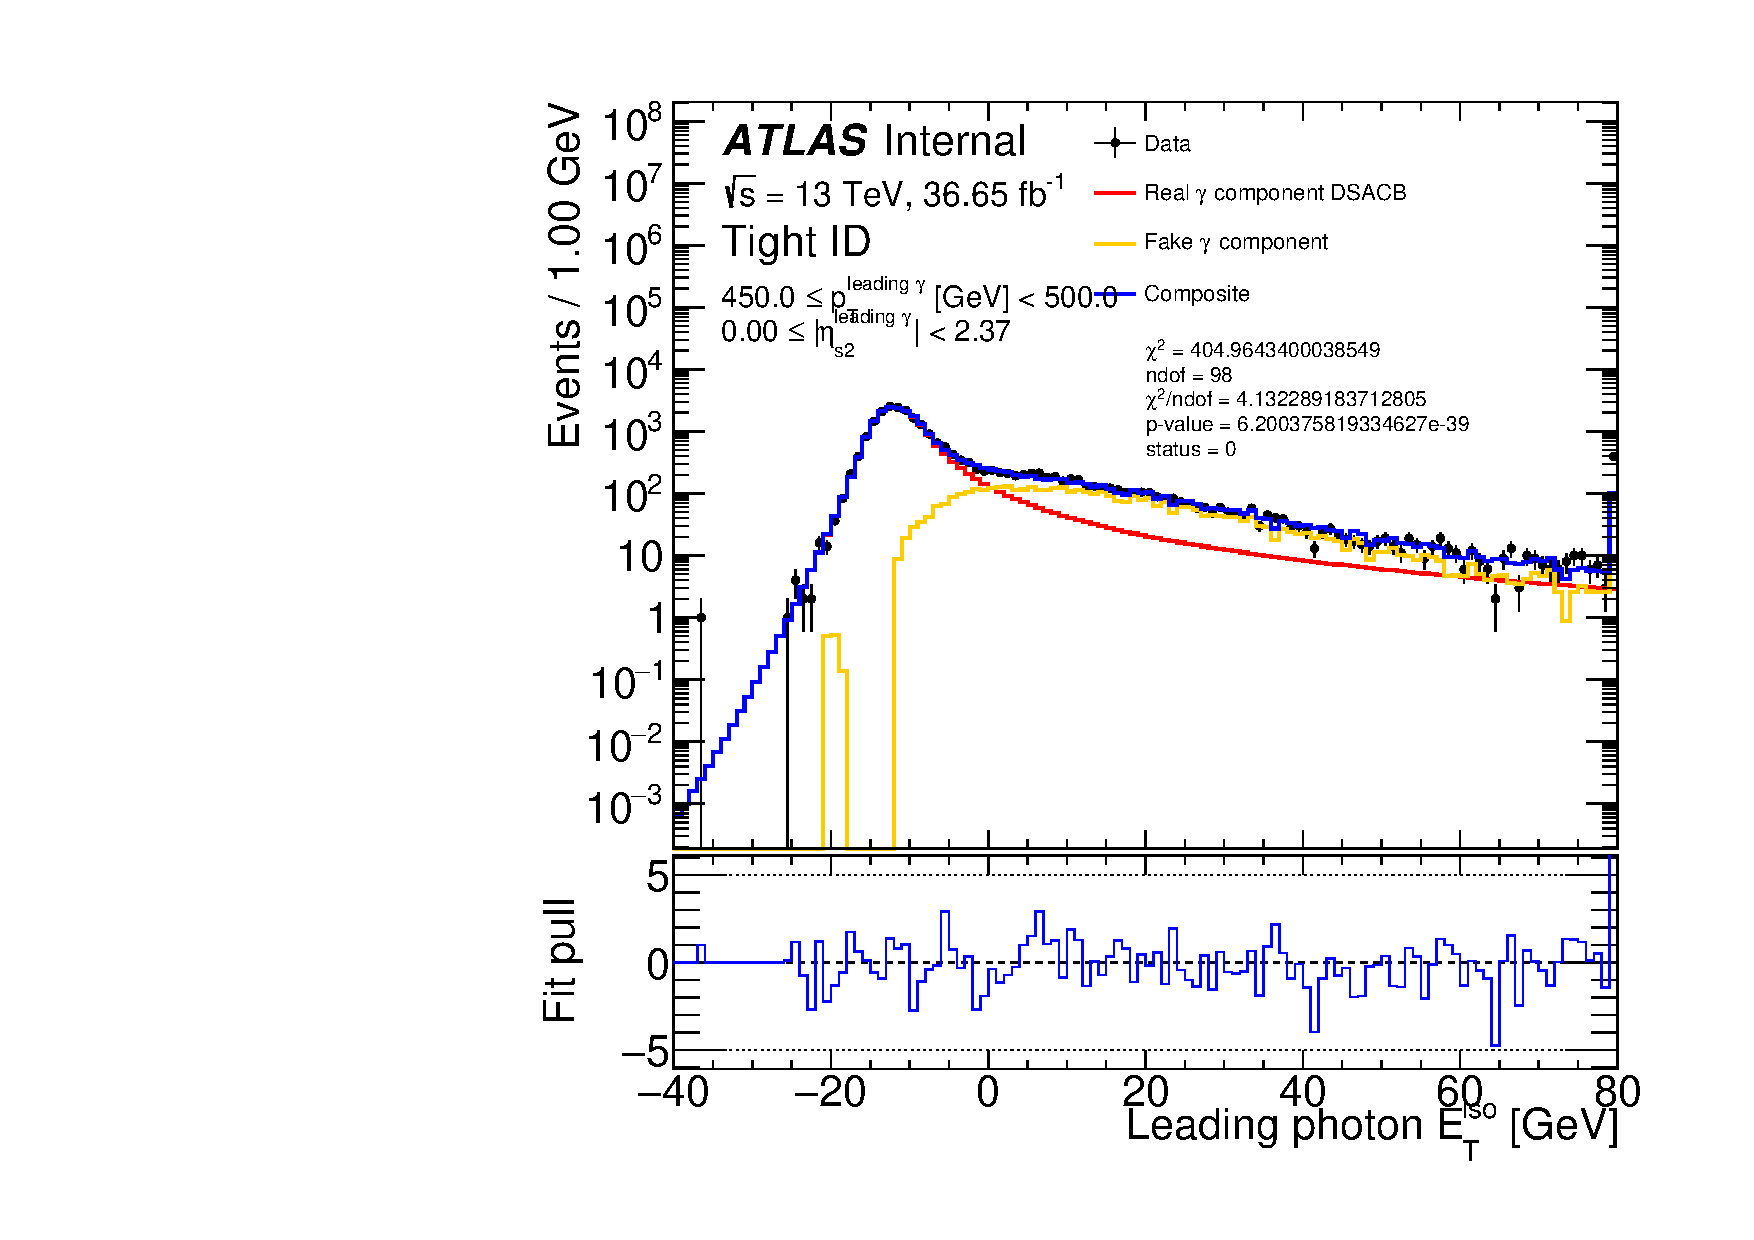
\includegraphics[width=\linewidth]{5_resonances/bkg/estimation/fits/lpid4/2015_2016/lph_pt0/lph_pt0__450p0/data__tight__composite__lph_pt0__450p0__abslph_etas20__0p00}
                \caption{\(450 < \ptgam < 500~\gev\).}
            \end{subfigure}
            \begin{subfigure}[h]{0.32\linewidth}
                \centering
                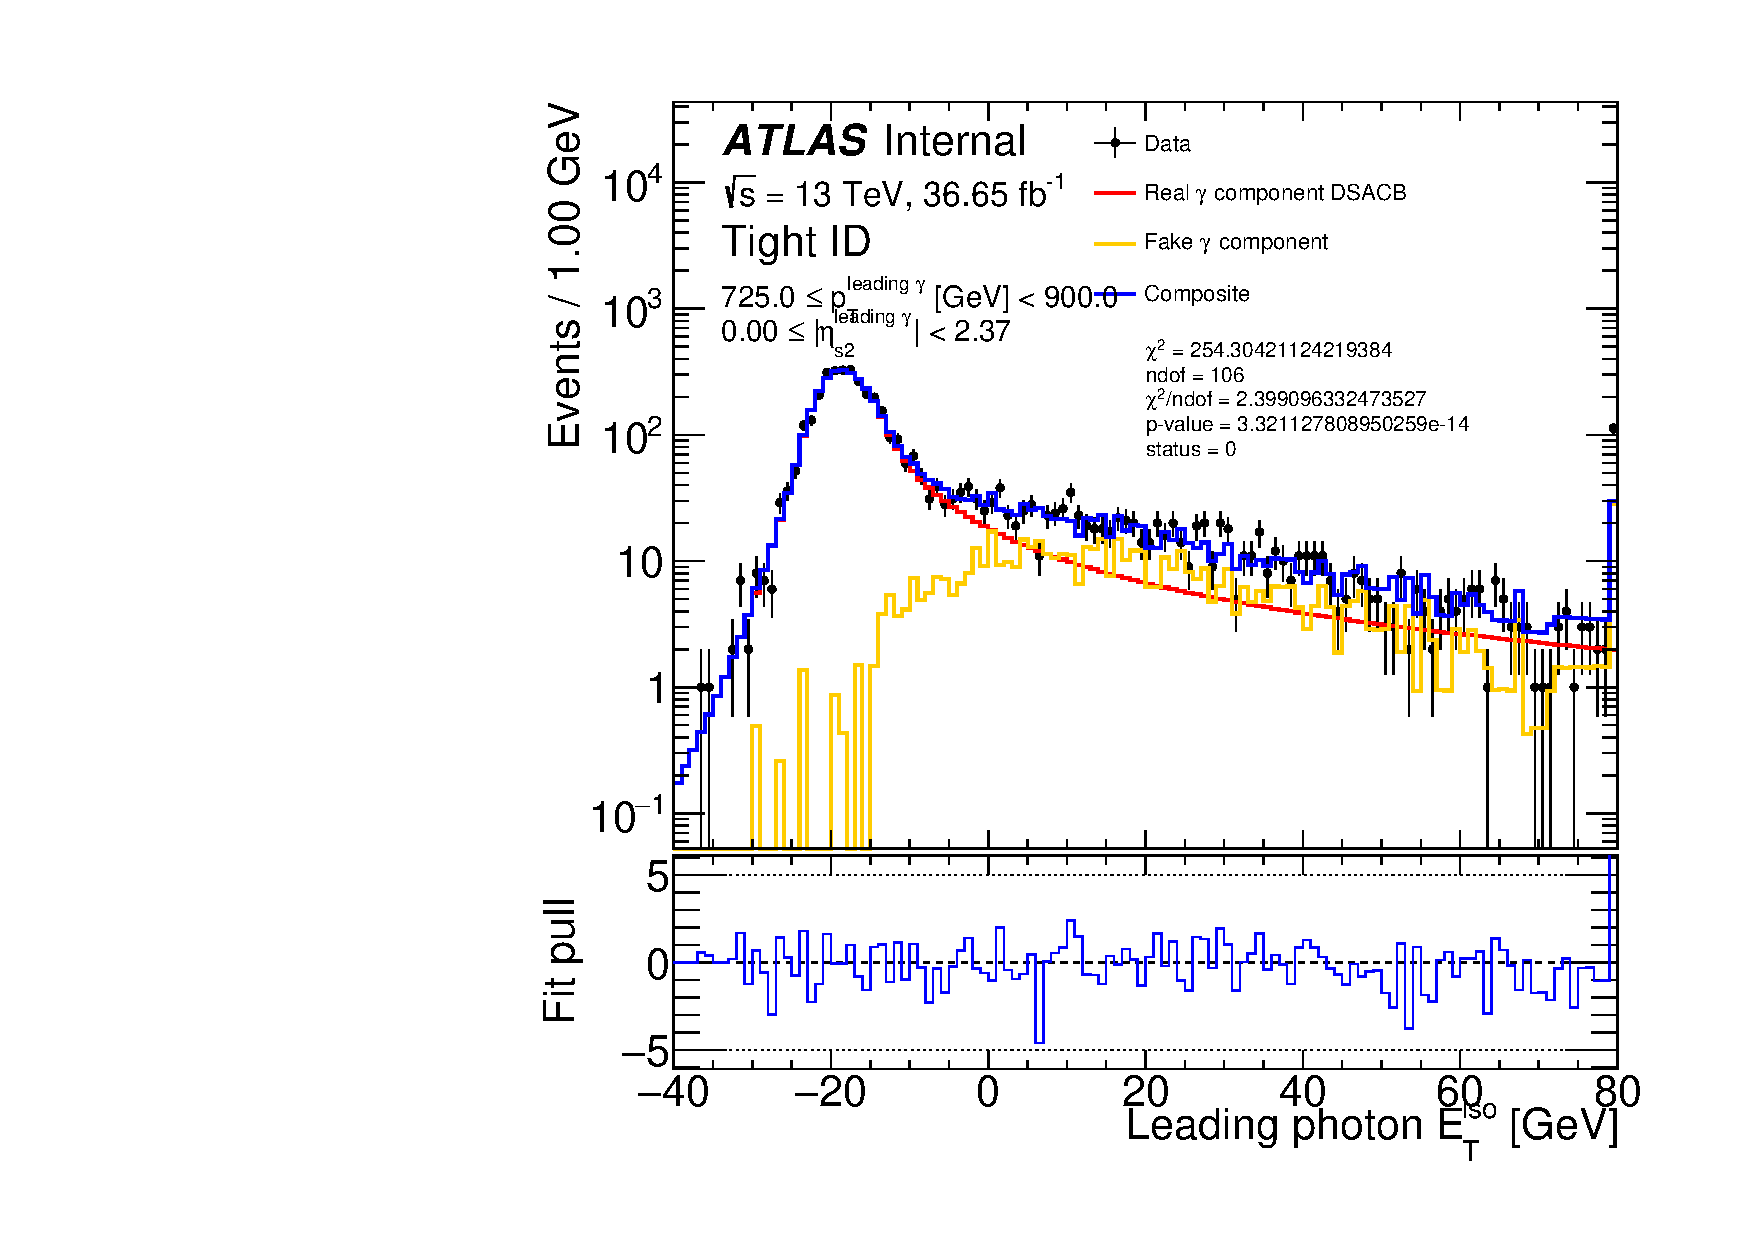
\includegraphics[width=\linewidth]{5_resonances/bkg/estimation/fits/lpid4/2015_2016/lph_pt0/lph_pt0__725p0/data__tight__composite__lph_pt0__725p0__abslph_etas20__0p00}
                \caption{\(725 < \ptgam < 900~\gev\).}
            \end{subfigure}
            \caption{Composite fit to data. The red curve represents the real photons component which is represented by a \ac{DSACB} distribution, computed in the first step. The yellow histogram is the fake photon contribution, obtained via leak-photon subtraction in the previous step. The lower pad of the figures represent the normalised residuals (or pull) of the fits.}
            \label{fig:bkg:estimation:fits_tightID_data}
        \end{figure}
\end{enumerate}





\subsection{Results}
\label{subsec:bkg:estimation:results}

From the above procedure using the ABCD and the template-fit methods, several key figures can be extracted. One important variable, to gain understanding of the phyiscs process, is the \gammajet purity, calculated as:
\[
    P_A = \frac{
        N^{A}_{\text{real}\gamma, \text{postfit}}
    }{
        N^{A}_{\text{real}\gamma, \text{postfit}} + N^{A}_{\text{fake}\gamma, \text{postfit}}
    }.
\]
These purities are shwon in \Fig{\ref{fig:bkg:estimation:results:results:purities}} and their numerical values in \Tab{\ref{tab:bkg:estimation:results:ffiso_purity_values}}. As it can be observed, purities of \(>92\%\) are achieved throughout the whole \ptgam range, indicating that processes containing a real photon and a jet encompass the majority of the sample.The purity measurements are smoothed using a \(3^{\text{rd}}\) order spline, shown with the red line in the figure.

\begin{table}[ht!]
    \caption{Smoothed photon fake factors \ffiso and \gammajet purity as a function of \ptgam.}
    \begin{tabular}{lcc}
        \toprule
        \(p_{T}^{\text{leading} \gamma}\) [GeV] & \(FF_{\text{iso}}\) &  Purity real \(\gamma\) in A \\
        \midrule
        $150-200$    & $0.1873$ & $0.9201$ \\
        $200-250$    & $0.1885$ & $0.9321$ \\
        $250-300$    & $0.1901$ & $0.9418$ \\
        $300-350$    & $0.1918$ & $0.9494$ \\
        $350-400$    & $0.1934$ & $0.9552$ \\
        $400-450$    & $0.1948$ & $0.9593$ \\
        $450-500$    & $0.1956$ & $0.9620$ \\
        $500-550$    & $0.1956$ & $0.9636$ \\
        $550-625$    & $0.1943$ & $0.9642$ \\
        $625-725$    & $0.1891$ & $0.9633$ \\
        $725-900$    & $0.1703$ & $0.9604$ \\
        $900-\infty$ & $0.0835$ & $0.9650$ \\
        \bottomrule
    \end{tabular}
    \label{tab:bkg:estimation:results:ffiso_purity_values}
    \centering
\end{table}
% \begin{table}[ht!]
%     \caption{Smoothed photon fake factors \ffiso and \gammajet purity as a function of \ptgam.}
%     \begin{tabular}{|l|c|c|c|c|}
%         \hline
%         \(p_{T}^{\text{leading} \gamma}\) [GeV] & \(FF_{\text{iso}}\) & Total \(FF_{\text{iso}}\) Unc. & Purity real \(\gamma\) in A & Total \(P_{A}\) Unc. \\
%         \hline
%         \hline
%         $150-200$ & $0.1873$ & $^{+0.0788 (42.10 \%)}_{-0.0719 (38.38 \%)}$ & $0.9201$ & $^{+0.0338 (3.67 \%)}_{-0.0113 (1.23 \%)}$ \\
%         \hline
%         $200-250$ & $0.1885$ & $^{+0.0640 (33.97 \%)}_{-0.0681 (36.14 \%)}$ & $0.9321$ & $^{+0.0252 (2.71 \%)}_{-0.0105 (1.13 \%)}$ \\
%         \hline
%         $250-300$ & $0.1901$ & $^{+0.0517 (27.22 \%)}_{-0.0641 (33.70 \%)}$ & $0.9418$ & $^{+0.0187 (1.99 \%)}_{-0.0101 (1.07 \%)}$ \\
%         \hline
%         $300-350$ & $0.1918$ & $^{+0.0418 (21.79 \%)}_{-0.0598 (31.18 \%)}$ & $0.9494$ & $^{+0.0141 (1.48 \%)}_{-0.0100 (1.06 \%)}$ \\
%         \hline
%         $350-400$ & $0.1934$ & $^{+0.0340 (17.57 \%)}_{-0.0554 (28.64 \%)}$ & $0.9552$ & $^{+0.0112 (1.17 \%)}_{-0.0103 (1.08 \%)}$ \\
%         \hline
%         $400-450$ & $0.1948$ & $^{+0.0281 (14.45 \%)}_{-0.0509 (26.15 \%)}$ & $0.9593$ & $^{+0.0097 (1.01 \%)}_{-0.0109 (1.13 \%)}$ \\
%         \hline
%         $450-500$ & $0.1956$ & $^{+0.0241 (12.30 \%)}_{-0.0465 (23.79 \%)}$ & $0.9620$ & $^{+0.0096 (0.99 \%)}_{-0.0117 (1.22 \%)}$ \\
%         \hline
%         $500-550$ & $0.1956$ & $^{+0.0215 (11.01 \%)}_{-0.0422 (21.58 \%)}$ & $0.9636$ & $^{+0.0105 (1.09 \%)}_{-0.0128 (1.33 \%)}$ \\
%         \hline
%         $550-625$ & $0.1943$ & $^{+0.0203 (10.45 \%)}_{-0.0371 (19.11 \%)}$ & $0.9642$ & $^{+0.0130 (1.34 \%)}_{-0.0146 (1.51 \%)}$ \\
%         \hline
%         $625-725$ & $0.1891$ & $^{+0.0215 (11.37 \%)}_{-0.0309 (16.32 \%)}$ & $0.9633$ & $^{+0.0180 (1.87 \%)}_{-0.0177 (1.84 \%)}$ \\
%         \hline
%         $725-900$ & $0.1703$ & $^{+0.0280 (16.42 \%)}_{-0.0239 (14.06 \%)}$ & $0.9604$ & $^{+0.0277 (2.88 \%)}_{-0.0238 (2.47 \%)}$ \\
%         \hline
%         $900-\infty$ & $0.0835$ & $^{+0.0428 (51.28 \%)}_{-0.0265 (31.72 \%)}$ & $0.9650$ & $^{+0.0384 (3.98 \%)}_{-0.0383 (3.97 \%)}$ \\
%         \hline
%     \end{tabular}
%     \label{tab:bkg:estimation:results:ffiso_purity_values}
%     \centering
% \end{table}

\begin{figure}[ht!]
    \centering
    \begin{subfigure}[h]{0.49\linewidth}
        \centering
        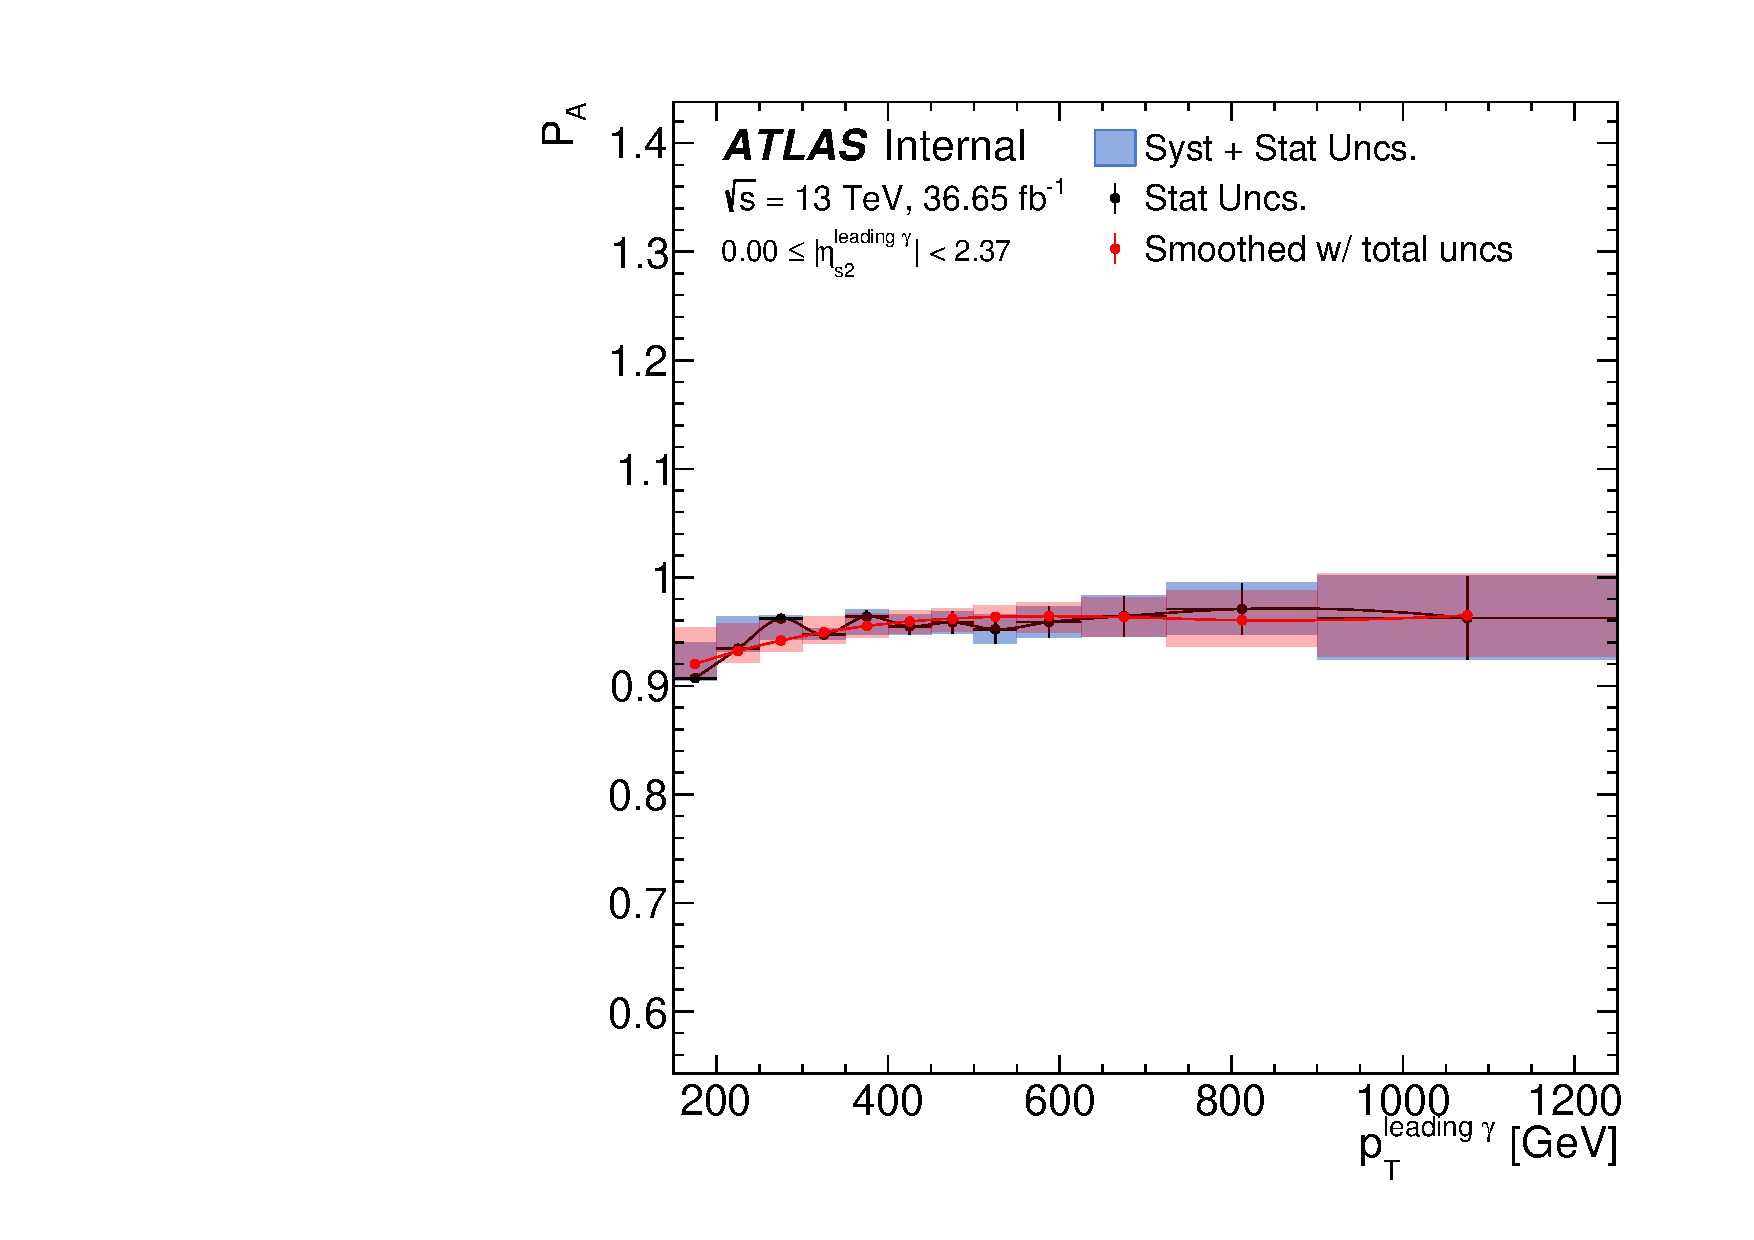
\includegraphics[width=\linewidth]{5_resonances/bkg/estimation/coefficients/can__purity_real_A__withsysts__lph_pt0__abslph_etas20_abslph_etas20__0p00__2015_2016}
        \caption{\(P_A\).}
        \label{fig:bkg:estimation:results:results:purities}
    \end{subfigure}
    \hfill
    \begin{subfigure}[h]{0.49\linewidth}
        \centering
        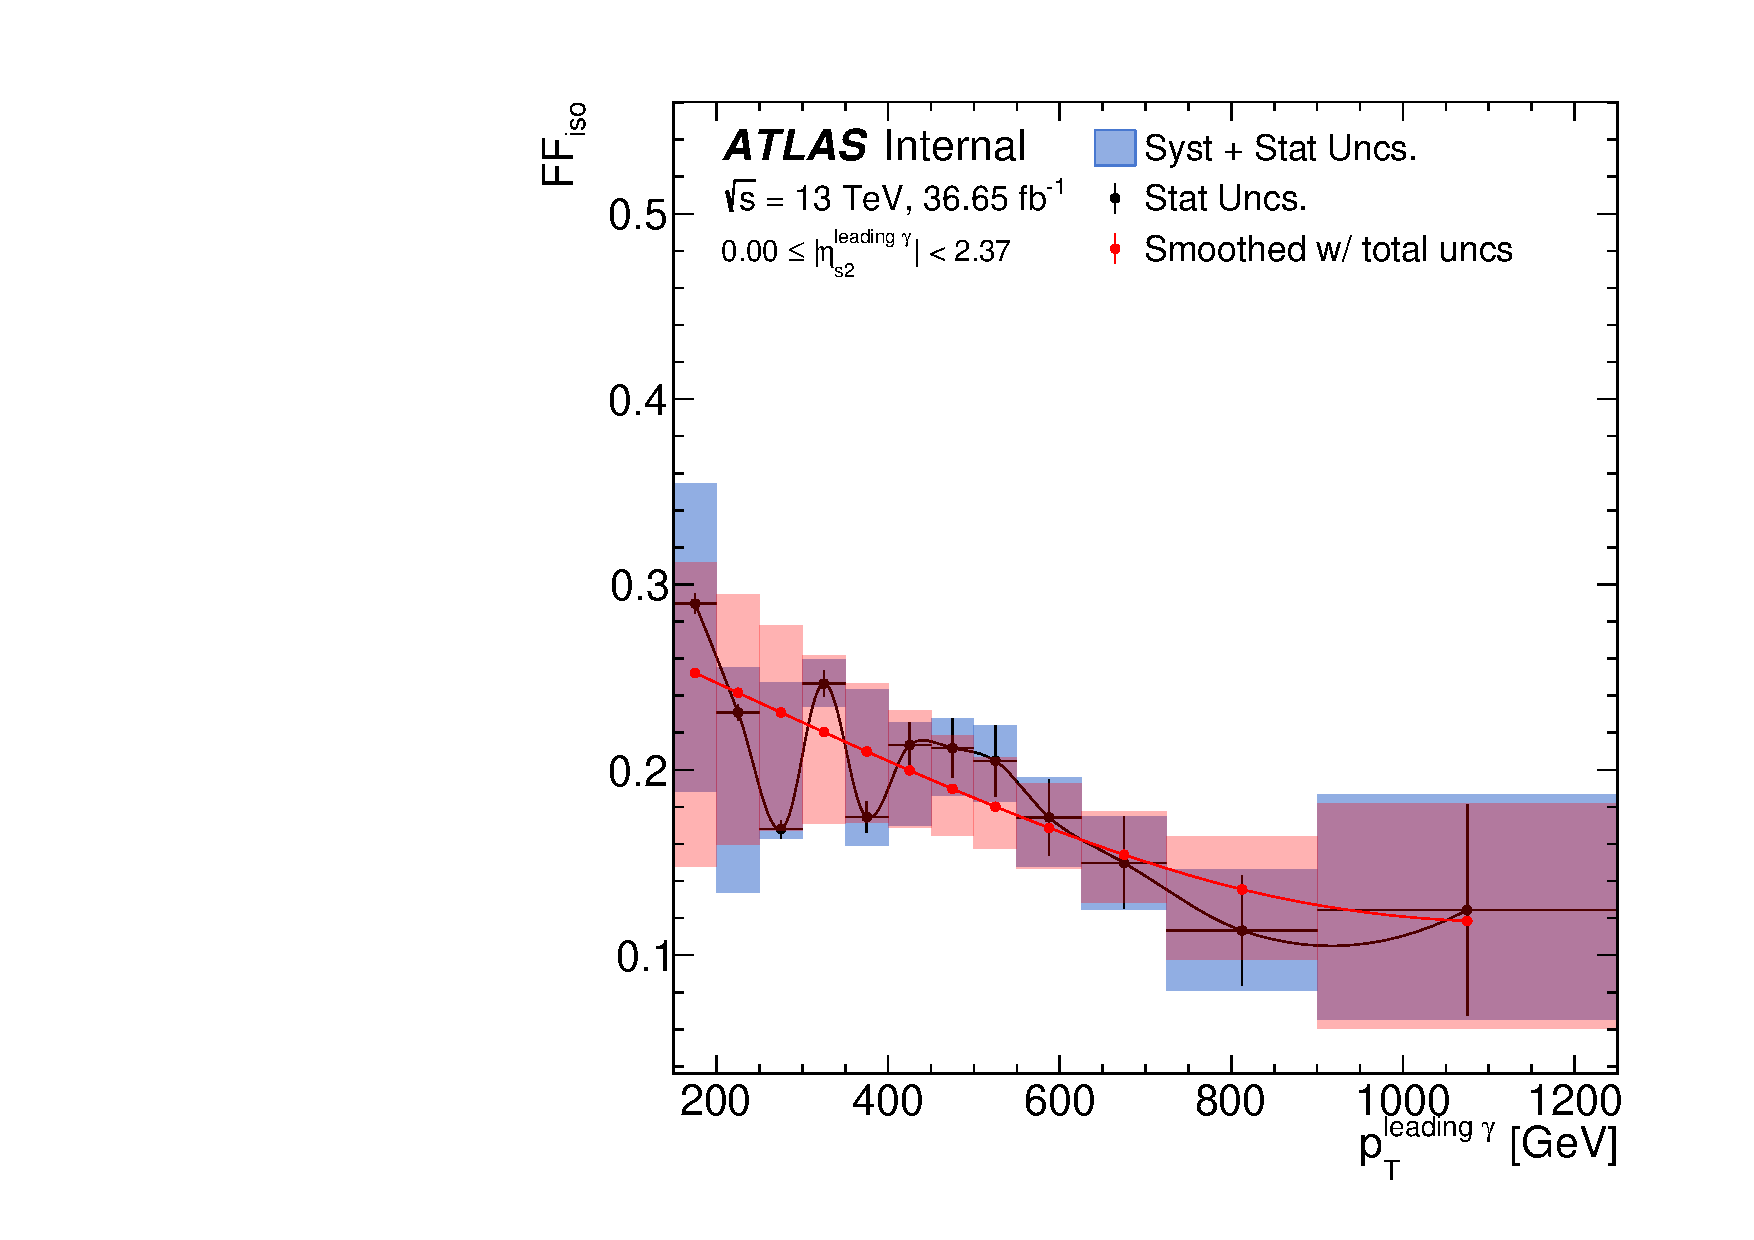
\includegraphics[width=\linewidth]{5_resonances/bkg/estimation/coefficients/can__FF_iso__withsysts__lph_pt0__abslph_etas20_abslph_etas20__0p00__2015_2016}
        \caption{\ffiso.}
        \label{fig:bkg:estimation:results:results:ffiso}
    \end{subfigure}
    \caption{Measured \gammajet \(P_A\) values (left) and \ffiso (right) as a function of \ptgam obtained using the ABCD method. The measurements are shown in black (statistical uncertainty only), the shaded blue rectangles show the total uncertainty on the measurements (systematic and statistical added in quadrature), and the red points and line show the smoothed measurements with the total uncertainty.}
    \label{fig:bkg:estimation:results:results}
\end{figure}


\acp{FaF}, and particularly \ffiso, are applied to data events in a control region CRJ-R, which only differs from any signal region \(R\) in the analysis by requiring non-isolated photons. \ffiso values, then, can be interpreted as the probability that a jet fakes a photon in region \(R\), given the fake-rate in CRJ-R. The results are shown with the black dots in \Fig{\ref{fig:bkg:estimation:results:results:ffiso}} and the total uncertainties with the shaded blue areas. As it can be seen from these results, unstable \ffiso value are seen for \(\ptgam<400~\gev\).
A smoothing using a \(3^{\text{rd}}\) order spline is employed in this case to avoid possible bumps in the final distributions. The numerical values of the \ffiso are shown in \Tab{\ref{tab:bkg:estimation:results:ffiso_purity_values}}.